\documentclass[border=8pt]{standalone}
\usepackage[UTF8]{ctex}
\usepackage{tikz}
\usetikzlibrary{arrows.meta}
\usepackage{array}
\usepackage{xcolor}
\begin{document}
\begin{minipage}{37.8cm}
\begin{center}
{\Large\bfseries Bench DAG 设计总览：先定形态，再配数据集}\\[3pt]
{\small 圆形节点表示 MFE operator；绿色为起点，红色为终点；蓝框为基础形态，红框为复杂综合形态。}\\[8pt]
{\normalsize\bfseries 基础形态（由简单到复杂）}\\[4pt]
\setlength{\tabcolsep}{6pt}
\renewcommand{\arraystretch}{1.18}
\begin{tabular}{*{5}{>{\centering\arraybackslash}p{7.16cm}}}
\fcolorbox{blue!65!black}{blue!2}{\begin{minipage}[t]{6.81cm}
\centering
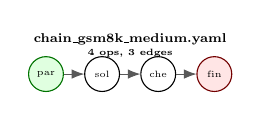
\begin{tikzpicture}[>=Latex, scale=0.66, transform shape,
  op/.style={circle, draw, align=center, minimum size=6.7mm, inner sep=0pt, font=\tiny, fill=white},
  start/.style={op, fill=green!12, draw=green!45!black},
  end/.style={op, fill=red!10, draw=red!45!black},
  startend/.style={op, fill=yellow!16, draw=orange!55!black},
  edge/.style={->, line width=0.35pt, draw=black!65}
]
\node[font=\scriptsize\bfseries, align=center] at (1.62,0.55) {chain\_gsm8k\_medium.yaml\\[-1pt]{\tiny 4 ops, 3 edges}};
\node[start] (n0) at (0.00,-0.00) {par};
\node[op] (n1) at (1.08,-0.00) {sol};
\node[op] (n2) at (2.16,-0.00) {che};
\node[end] (n3) at (3.24,-0.00) {fin};
\draw[edge] (n2) -- (n3);
\draw[edge] (n0) -- (n1);
\draw[edge] (n1) -- (n2);
\end{tikzpicture}
\\[-2pt]
{\scriptsize\bfseries 形态：线性链式推理}\\
{\scriptsize\bfseries 数据集：GSM8K}\\[-1pt]
{\scriptsize 小学数学文字题，天然适合 parse、solve、check 的短链式逐步推理。}
\end{minipage}}
&
\fcolorbox{blue!65!black}{blue!2}{\begin{minipage}[t]{6.81cm}
\centering
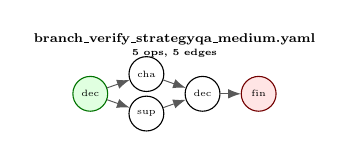
\begin{tikzpicture}[>=Latex, scale=0.66, transform shape,
  op/.style={circle, draw, align=center, minimum size=6.7mm, inner sep=0pt, font=\tiny, fill=white},
  start/.style={op, fill=green!12, draw=green!45!black},
  end/.style={op, fill=red!10, draw=red!45!black},
  startend/.style={op, fill=yellow!16, draw=orange!55!black},
  edge/.style={->, line width=0.35pt, draw=black!65}
]
\node[font=\scriptsize\bfseries, align=center] at (1.62,0.93) {branch\_verify\_strategyqa\_medium.yaml\\[-1pt]{\tiny 5 ops, 5 edges}};
\node[start] (n0) at (0.00,-0.00) {dec};
\node[op] (n1) at (1.08,-0.38) {sup};
\node[op] (n2) at (1.08,0.38) {cha};
\node[op] (n3) at (2.16,-0.00) {dec};
\node[end] (n4) at (3.24,-0.00) {fin};
\draw[edge] (n2) -- (n3);
\draw[edge] (n3) -- (n4);
\draw[edge] (n0) -- (n2);
\draw[edge] (n0) -- (n1);
\draw[edge] (n1) -- (n3);
\end{tikzpicture}
\\[-2pt]
{\scriptsize\bfseries 形态：隐式分解 + 双分支校验}\\
{\scriptsize\bfseries 数据集：StrategyQA}\\[-1pt]
{\scriptsize 隐式多步 yes/no 常识题；支持/反驳两条路径能暴露隐藏假设。}
\end{minipage}}
&
\fcolorbox{blue!65!black}{blue!2}{\begin{minipage}[t]{6.81cm}
\centering
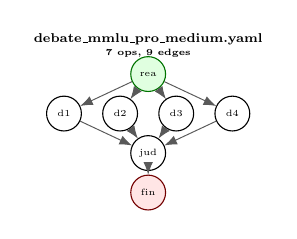
\begin{tikzpicture}[>=Latex, scale=0.66, transform shape,
  op/.style={circle, draw, align=center, minimum size=6.7mm, inner sep=0pt, font=\tiny, fill=white},
  start/.style={op, fill=green!12, draw=green!45!black},
  end/.style={op, fill=red!10, draw=red!45!black},
  startend/.style={op, fill=yellow!16, draw=orange!55!black},
  edge/.style={->, line width=0.35pt, draw=black!65}
]
\node[font=\scriptsize\bfseries, align=center] at (0.00,0.55) {debate\_mmlu\_pro\_medium.yaml\\[-1pt]{\tiny 7 ops, 9 edges}};
\node[start] (n0) at (0.00,0.00) {rea};
\node[op] (n1) at (-1.62,-0.76) {d1};
\node[op] (n2) at (-0.54,-0.76) {d2};
\node[op] (n3) at (0.54,-0.76) {d3};
\node[op] (n4) at (1.62,-0.76) {d4};
\node[op] (n5) at (0.00,-1.52) {jud};
\node[end] (n6) at (0.00,-2.28) {fin};
\draw[edge] (n1) -- (n5);
\draw[edge] (n2) -- (n5);
\draw[edge] (n3) -- (n5);
\draw[edge] (n4) -- (n5);
\draw[edge] (n5) -- (n6);
\draw[edge] (n0) -- (n1);
\draw[edge] (n0) -- (n2);
\draw[edge] (n0) -- (n3);
\draw[edge] (n0) -- (n4);
\end{tikzpicture}
\\[-2pt]
{\scriptsize\bfseries 形态：多路并行辩论 + 裁决}\\
{\scriptsize\bfseries 数据集：MMLU-Pro}\\[-1pt]
{\scriptsize 更难的多任务选择题；多名 debater 并行给出候选答案，再由 judge 裁决。}
\end{minipage}}
&
\fcolorbox{blue!65!black}{blue!2}{\begin{minipage}[t]{6.81cm}
\centering
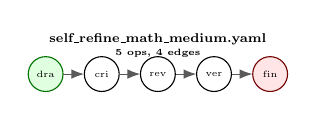
\begin{tikzpicture}[>=Latex, scale=0.66, transform shape,
  op/.style={circle, draw, align=center, minimum size=6.7mm, inner sep=0pt, font=\tiny, fill=white},
  start/.style={op, fill=green!12, draw=green!45!black},
  end/.style={op, fill=red!10, draw=red!45!black},
  startend/.style={op, fill=yellow!16, draw=orange!55!black},
  edge/.style={->, line width=0.35pt, draw=black!65}
]
\node[font=\scriptsize\bfseries, align=center] at (2.16,0.55) {self\_refine\_math\_medium.yaml\\[-1pt]{\tiny 5 ops, 4 edges}};
\node[start] (n0) at (0.00,-0.00) {dra};
\node[op] (n1) at (1.08,-0.00) {cri};
\node[op] (n2) at (2.16,-0.00) {rev};
\node[op] (n3) at (3.24,-0.00) {ver};
\node[end] (n4) at (4.32,-0.00) {fin};
\draw[edge] (n1) -- (n2);
\draw[edge] (n0) -- (n1);
\draw[edge] (n2) -- (n3);
\draw[edge] (n3) -- (n4);
\end{tikzpicture}
\\[-2pt]
{\scriptsize\bfseries 形态：草稿 - 批改 - 修正}\\
{\scriptsize\bfseries 数据集：MATH}\\[-1pt]
{\scriptsize 竞赛数学题更容易出现推导漏洞，适合用批改和修正节点提高稳健性。}
\end{minipage}}
&
\fcolorbox{blue!65!black}{blue!2}{\begin{minipage}[t]{6.81cm}
\centering
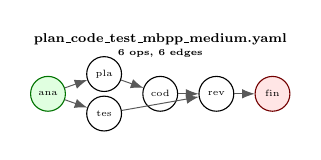
\begin{tikzpicture}[>=Latex, scale=0.66, transform shape,
  op/.style={circle, draw, align=center, minimum size=6.7mm, inner sep=0pt, font=\tiny, fill=white},
  start/.style={op, fill=green!12, draw=green!45!black},
  end/.style={op, fill=red!10, draw=red!45!black},
  startend/.style={op, fill=yellow!16, draw=orange!55!black},
  edge/.style={->, line width=0.35pt, draw=black!65}
]
\node[font=\scriptsize\bfseries, align=center] at (2.16,0.93) {plan\_code\_test\_mbpp\_medium.yaml\\[-1pt]{\tiny 6 ops, 6 edges}};
\node[start] (n0) at (0.00,-0.00) {ana};
\node[op] (n1) at (1.08,0.38) {pla};
\node[op] (n2) at (1.08,-0.38) {tes};
\node[op] (n3) at (2.16,-0.00) {cod};
\node[op] (n4) at (3.24,-0.00) {rev};
\node[end] (n5) at (4.32,-0.00) {fin};
\draw[edge] (n0) -- (n1);
\draw[edge] (n0) -- (n2);
\draw[edge] (n3) -- (n4);
\draw[edge] (n1) -- (n3);
\draw[edge] (n4) -- (n5);
\draw[edge] (n2) -- (n4);
\end{tikzpicture}
\\[-2pt]
{\scriptsize\bfseries 形态：计划 - 代码 - 测试}\\
{\scriptsize\bfseries 数据集：MBPP}\\[-1pt]
{\scriptsize 小型 Python 编程题带自然语言需求和测试，适合计划、实现、测试审查。}
\end{minipage}}\\[12pt]
\end{tabular}
\\[2pt]
{\normalsize\bfseries 复杂综合形态（尽量覆盖上面的结构特征）}\\[4pt]
\begin{tabular}{*{2}{>{\centering\arraybackslash}p{17.95cm}}}
\fcolorbox{red!72!black}{red!2}{\begin{minipage}[t]{17.60cm}
\centering
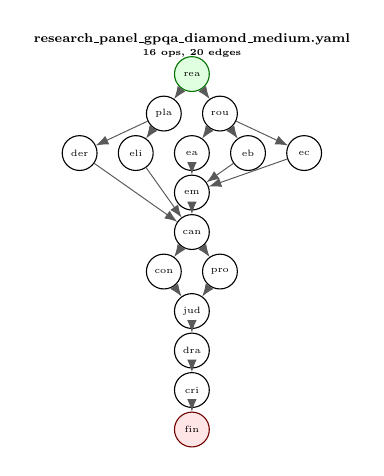
\begin{tikzpicture}[>=Latex, scale=0.66, transform shape,
  op/.style={circle, draw, align=center, minimum size=6.7mm, inner sep=0pt, font=\tiny, fill=white},
  start/.style={op, fill=green!12, draw=green!45!black},
  end/.style={op, fill=red!10, draw=red!45!black},
  startend/.style={op, fill=yellow!16, draw=orange!55!black},
  edge/.style={->, line width=0.35pt, draw=black!65}
]
\node[font=\scriptsize\bfseries, align=center] at (0.00,0.55) {research\_panel\_gpqa\_diamond\_medium.yaml\\[-1pt]{\tiny 16 ops, 20 edges}};
\node[start] (n0) at (0.00,0.00) {rea};
\node[op] (n1) at (0.54,-0.76) {rou};
\node[op] (n2) at (-0.54,-0.76) {pla};
\node[op] (n3) at (0.00,-1.52) {ea};
\node[op] (n4) at (1.08,-1.52) {eb};
\node[op] (n5) at (2.16,-1.52) {ec};
\node[op] (n6) at (-2.16,-1.52) {der};
\node[op] (n7) at (-1.08,-1.52) {eli};
\node[op] (n8) at (0.00,-2.28) {em};
\node[op] (n9) at (0.00,-3.04) {can};
\node[op] (n10) at (0.54,-3.80) {pro};
\node[op] (n11) at (-0.54,-3.80) {con};
\node[op] (n12) at (0.00,-4.56) {jud};
\node[op] (n13) at (0.00,-5.32) {dra};
\node[op] (n14) at (0.00,-6.08) {cri};
\node[end] (n15) at (0.00,-6.84) {fin};
\draw[edge] (n9) -- (n11);
\draw[edge] (n9) -- (n10);
\draw[edge] (n11) -- (n12);
\draw[edge] (n14) -- (n15);
\draw[edge] (n6) -- (n9);
\draw[edge] (n13) -- (n14);
\draw[edge] (n7) -- (n9);
\draw[edge] (n8) -- (n9);
\draw[edge] (n3) -- (n8);
\draw[edge] (n4) -- (n8);
\draw[edge] (n5) -- (n8);
\draw[edge] (n12) -- (n13);
\draw[edge] (n2) -- (n6);
\draw[edge] (n2) -- (n7);
\draw[edge] (n10) -- (n12);
\draw[edge] (n0) -- (n2);
\draw[edge] (n0) -- (n1);
\draw[edge] (n1) -- (n3);
\draw[edge] (n1) -- (n4);
\draw[edge] (n1) -- (n5);
\end{tikzpicture}
\\[-2pt]
{\scriptsize\bfseries 形态：专家组 + 证据 + 辩论 + 反思}\\
{\scriptsize\bfseries 数据集：GPQA Diamond}\\[-1pt]
{\scriptsize 研究生级科学选择题，难度高，适合多专家证据、选项排除、辩论和反思。}
\end{minipage}}
&
\fcolorbox{red!72!black}{red!2}{\begin{minipage}[t]{17.60cm}
\centering
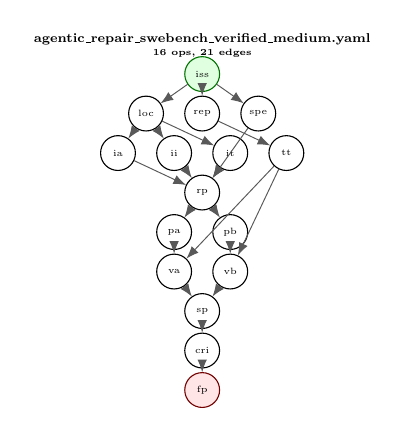
\begin{tikzpicture}[>=Latex, scale=0.66, transform shape,
  op/.style={circle, draw, align=center, minimum size=6.7mm, inner sep=0pt, font=\tiny, fill=white},
  start/.style={op, fill=green!12, draw=green!45!black},
  end/.style={op, fill=red!10, draw=red!45!black},
  startend/.style={op, fill=yellow!16, draw=orange!55!black},
  edge/.style={->, line width=0.35pt, draw=black!65}
]
\node[font=\scriptsize\bfseries, align=center] at (0.00,0.55) {agentic\_repair\_swebench\_verified\_medium.yaml\\[-1pt]{\tiny 16 ops, 21 edges}};
\node[start] (n0) at (0.00,0.00) {iss};
\node[op] (n1) at (0.00,-0.76) {rep};
\node[op] (n2) at (-1.08,-0.76) {loc};
\node[op] (n3) at (1.08,-0.76) {spe};
\node[op] (n4) at (-1.62,-1.52) {ia};
\node[op] (n5) at (0.54,-1.52) {it};
\node[op] (n6) at (-0.54,-1.52) {ii};
\node[op] (n7) at (1.62,-1.52) {tt};
\node[op] (n8) at (0.00,-2.28) {rp};
\node[op] (n9) at (-0.54,-3.04) {pa};
\node[op] (n10) at (0.54,-3.04) {pb};
\node[op] (n11) at (-0.54,-3.80) {va};
\node[op] (n12) at (0.54,-3.80) {vb};
\node[op] (n13) at (0.00,-4.56) {sp};
\node[op] (n14) at (0.00,-5.32) {cri};
\node[end] (n15) at (0.00,-6.08) {fp};
\draw[edge] (n14) -- (n15);
\draw[edge] (n4) -- (n8);
\draw[edge] (n6) -- (n8);
\draw[edge] (n5) -- (n8);
\draw[edge] (n0) -- (n2);
\draw[edge] (n0) -- (n1);
\draw[edge] (n0) -- (n3);
\draw[edge] (n2) -- (n4);
\draw[edge] (n2) -- (n6);
\draw[edge] (n2) -- (n5);
\draw[edge] (n9) -- (n11);
\draw[edge] (n10) -- (n12);
\draw[edge] (n8) -- (n9);
\draw[edge] (n8) -- (n10);
\draw[edge] (n1) -- (n7);
\draw[edge] (n13) -- (n14);
\draw[edge] (n3) -- (n8);
\draw[edge] (n7) -- (n11);
\draw[edge] (n7) -- (n12);
\draw[edge] (n11) -- (n13);
\draw[edge] (n12) -- (n13);
\end{tikzpicture}
\\[-2pt]
{\scriptsize\bfseries 形态：定位 + 双补丁 + 测试选择}\\
{\scriptsize\bfseries 数据集：SWE-bench Verified}\\[-1pt]
{\scriptsize 真实 GitHub issue 修复任务；需要定位、补丁候选、测试验证和回归风险检查。}
\end{minipage}}\\
\end{tabular}
\end{center}
\end{minipage}
\end{document}
